\section{Auswertung}
\label{sec:Auswertung}

Im Folgenden sollen mithilfe der oben genannten Messverfahren die Durchmesser der Störstellen in dem Acrylblock bestimmt werden
und anschließend anhand eines Brustmodells zwei Tumore identifiziert werden.

\subsection{Ausmessung des Acrylblocks mittels A-Scan} \label{sec:a-scan}

Mithilfe einer Schieblehre werden die Maße des Acrylblocks bestimmt und in \autoref{tab:acrylblock} dargestellt.
\begin{table}
  \centering
  \caption{Die Abmessungen des Acrylblocks.}
  \label{tab:acrylblock}
  \begin{tabular}{c c}
    \toprule
    & $s \mathbin{/} \unit{cm}$ \\
    \midrule
    Länge   & 15,0 \\
    Breite  &  4,0 \\
    Höhe    & 80,4 \\
    \bottomrule
  \end{tabular}
\end{table}
Der Ort einer Störstelle wird mittels A-Scan bestimmt, indem die Laufzeit jeweils vom oberen und unteren Ende des Acrylblocks zur Störstelle gemessen wird.
Dabei muss die Laufzeit aufgrund der Sonden-Schutzschicht der Dicke $\qty{0.2}{cm}$ angepasst werden.
Für die Berechnung der Abstände $d_\text{oben}$ und $d_\text{unten}$ wird eine Phasengeschwindigkeit in Acryl
von $\qty{2730}{\meter\per\second}$ mit dem Weg-Zeit-Gesetz nach \autoref{eq:wegzeit} verwendet.
Aus der Differenz der ausgemessenen Höhe des Acrylblocks und der berechneten Abstände ergeben sich in \autoref{tab:tiefenmessung} die Durchmesser der Störstellen $d_\text{Loch}$.

\begin{table}[H]
  \centering
  \caption{Die Laufzeiten und die berechneten Werte der Störstellen mittels A-Scan.}
  \label{tab:tiefenmessung}
  % \sisetup{table-format=1.2}
  \begin{tabular}{c c c c c c}
    \toprule
    \multicolumn{1}{c}{Stelle} &
    \multicolumn{1}{c}{$t_\text{oben} \mathbin{/} \unit{\micro\second}$} &
    \multicolumn{1}{c}{$d_\text{oben} \mathbin{/} \unit{\centi\meter}$} &
    \multicolumn{1}{c}{$t_\text{unten} \mathbin{/} \unit{\micro\second}$} &
    \multicolumn{1}{c}{$d_\text{unten} \mathbin{/} \unit{\centi\meter}$} &
    \multicolumn{1}{c}{$d_\text{Loch} \mathbin{/} \unit{\milli\meter}$} \\

    \cmidrule(lr){1-1} \cmidrule(lr){2-3} \cmidrule(lr){4-5} \cmidrule(lr){6-6} 
    
          3 &    46,5 &    6,35 &     10,7 &     1,46 &    4,32 \\
          4 &    40,4 &    5,51 &     17,5 &     2,39 &    3,37 \\
          5 &    35,0 &    4,78 &     23,0 &     3,14 &    3,23 \\
          6 &    28,5 &    3,89 &     29,4 &     4,01 &    3,37 \\
          7 &    23,5 &    3,21 &     35,5 &     4,85 &    1,86 \\
          8 &    16,0 &    2,18 &     40,8 &     5,57 &    4,87 \\
          9 &    13,0 &    1,77 &     46,6 &     6,36 &    1,05 \\
         10 &     6,5 &    0,89 &        - &        - &       - \\
         11 &    41,5 &    5,66 &     12,4 &     1,69 &    8,83 \\
    \bottomrule
  \end{tabular}
\end{table}

Eine beispielhafte Aufnahme eines solchen A-Scans einer Störstelle ist in \autoref{fig:a-scan} dargestellt.
\begin{figure}
  \centering
  
  \begin{subfigure}{0.49\columnwidth}
  \centering
  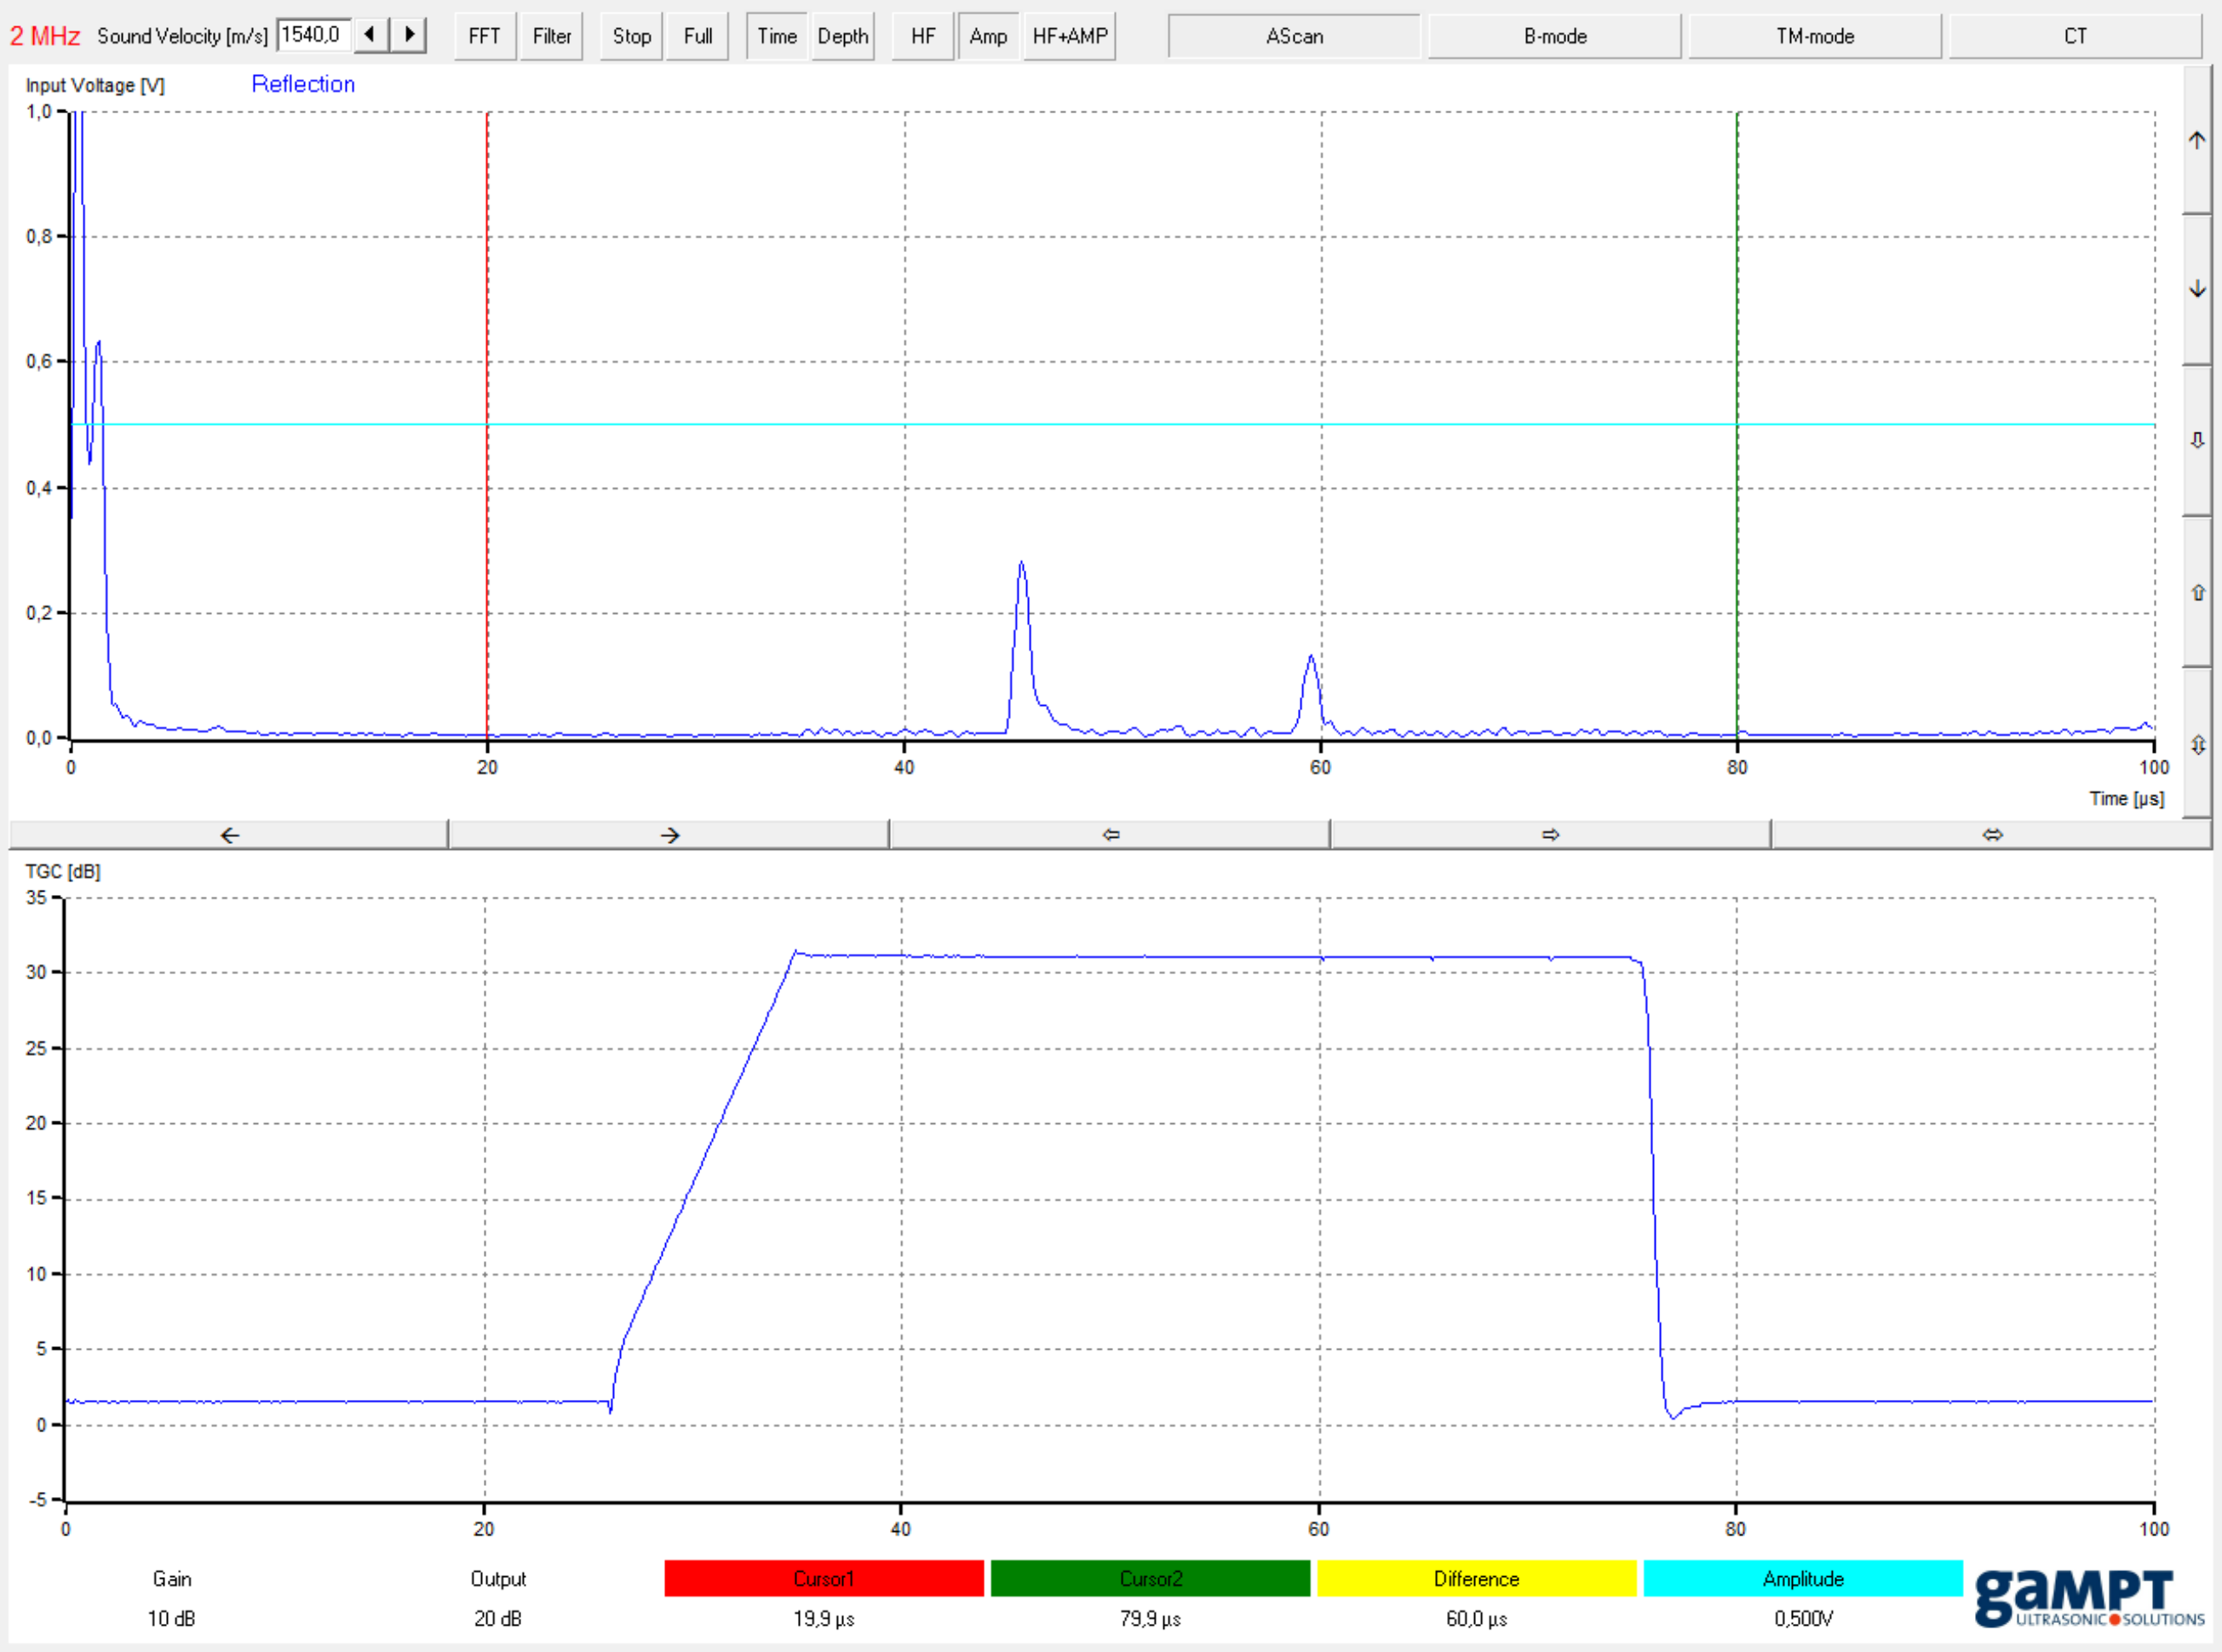
\includegraphics[width=\textwidth]{pictures/o3.png}
  \caption{A-Scan von oben.}
  \label{fig:o3}
  \end{subfigure}
  \hfill
  \begin{subfigure}{0.49\columnwidth}
  \centering
  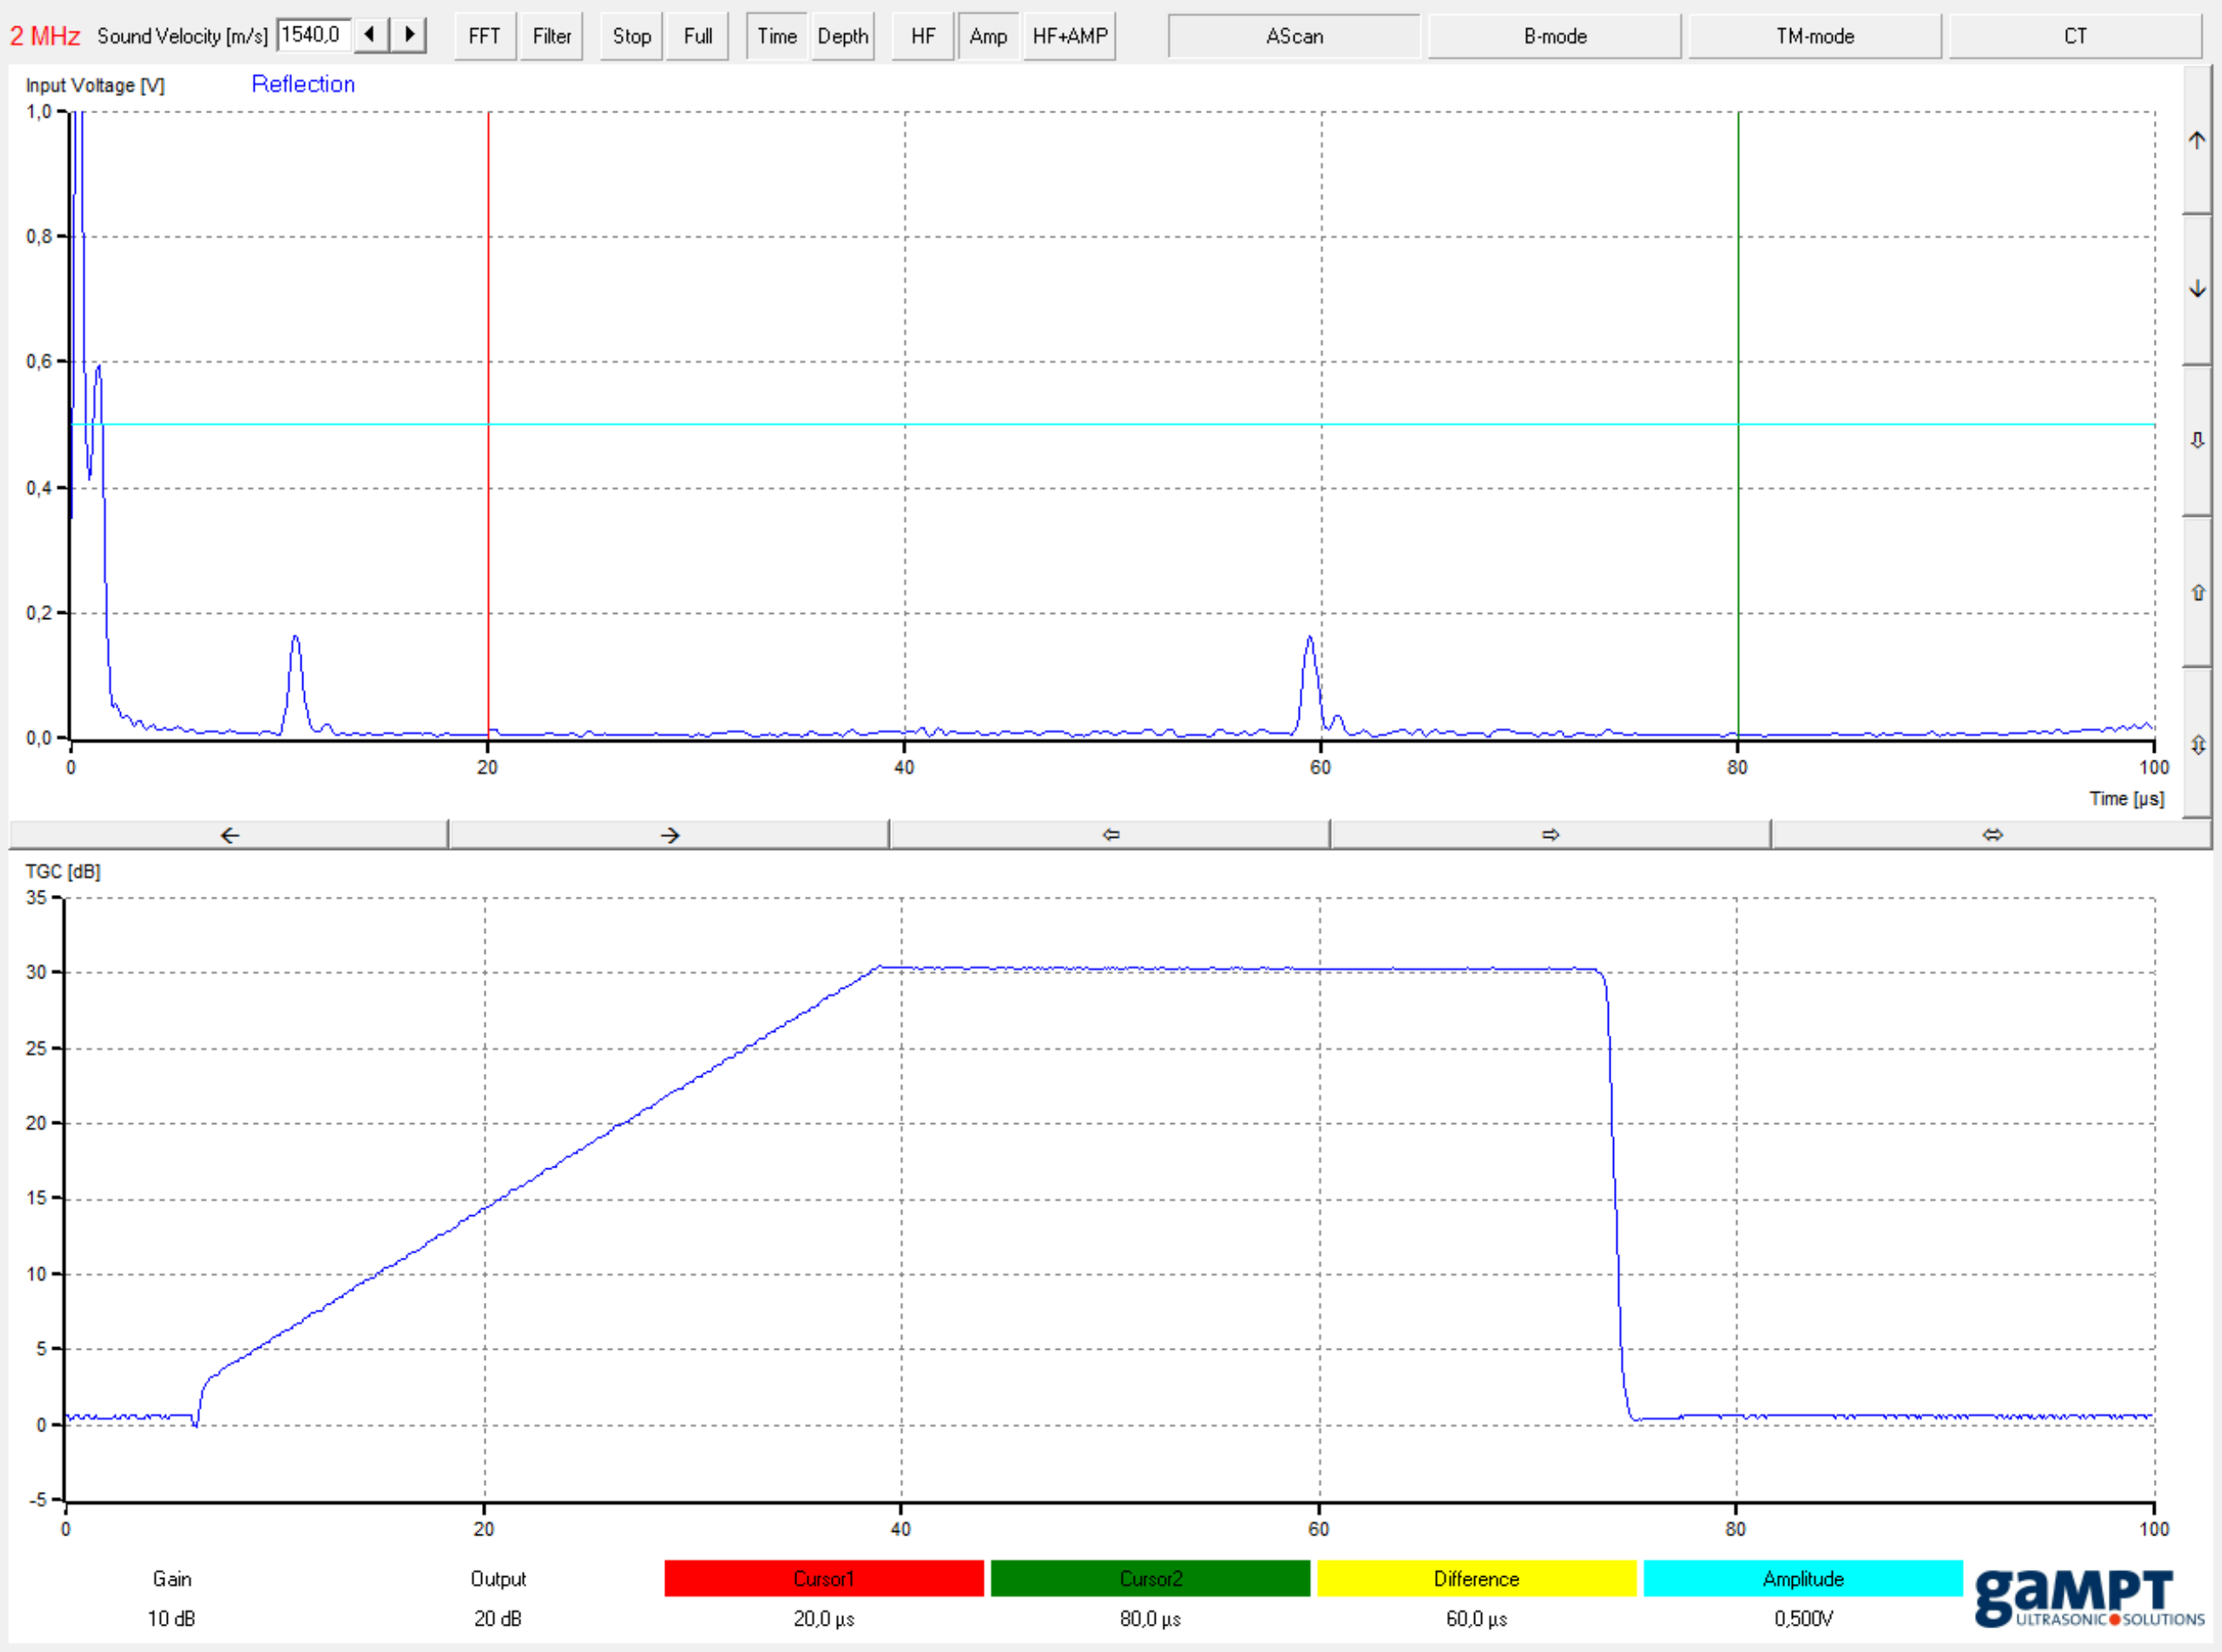
\includegraphics[width=\textwidth]{pictures/u3.png}
  \caption{A-Scan von unten.}
  \label{fig:u3}
  \end{subfigure}

  \caption{Beispielhafter A-Scan der Störstelle 3.}
  \label{fig:a-scan}
\end{figure}


\subsection{Ausmessung des Acrylblocks mittels B-Scan} \label{sec:b-scan}

Die Aufnahmen des B-Scans sind in \autoref{fig:b-scan} zu sehen.
\begin{figure}
  \centering
  
  \begin{subfigure}{0.49\columnwidth}
  \centering
  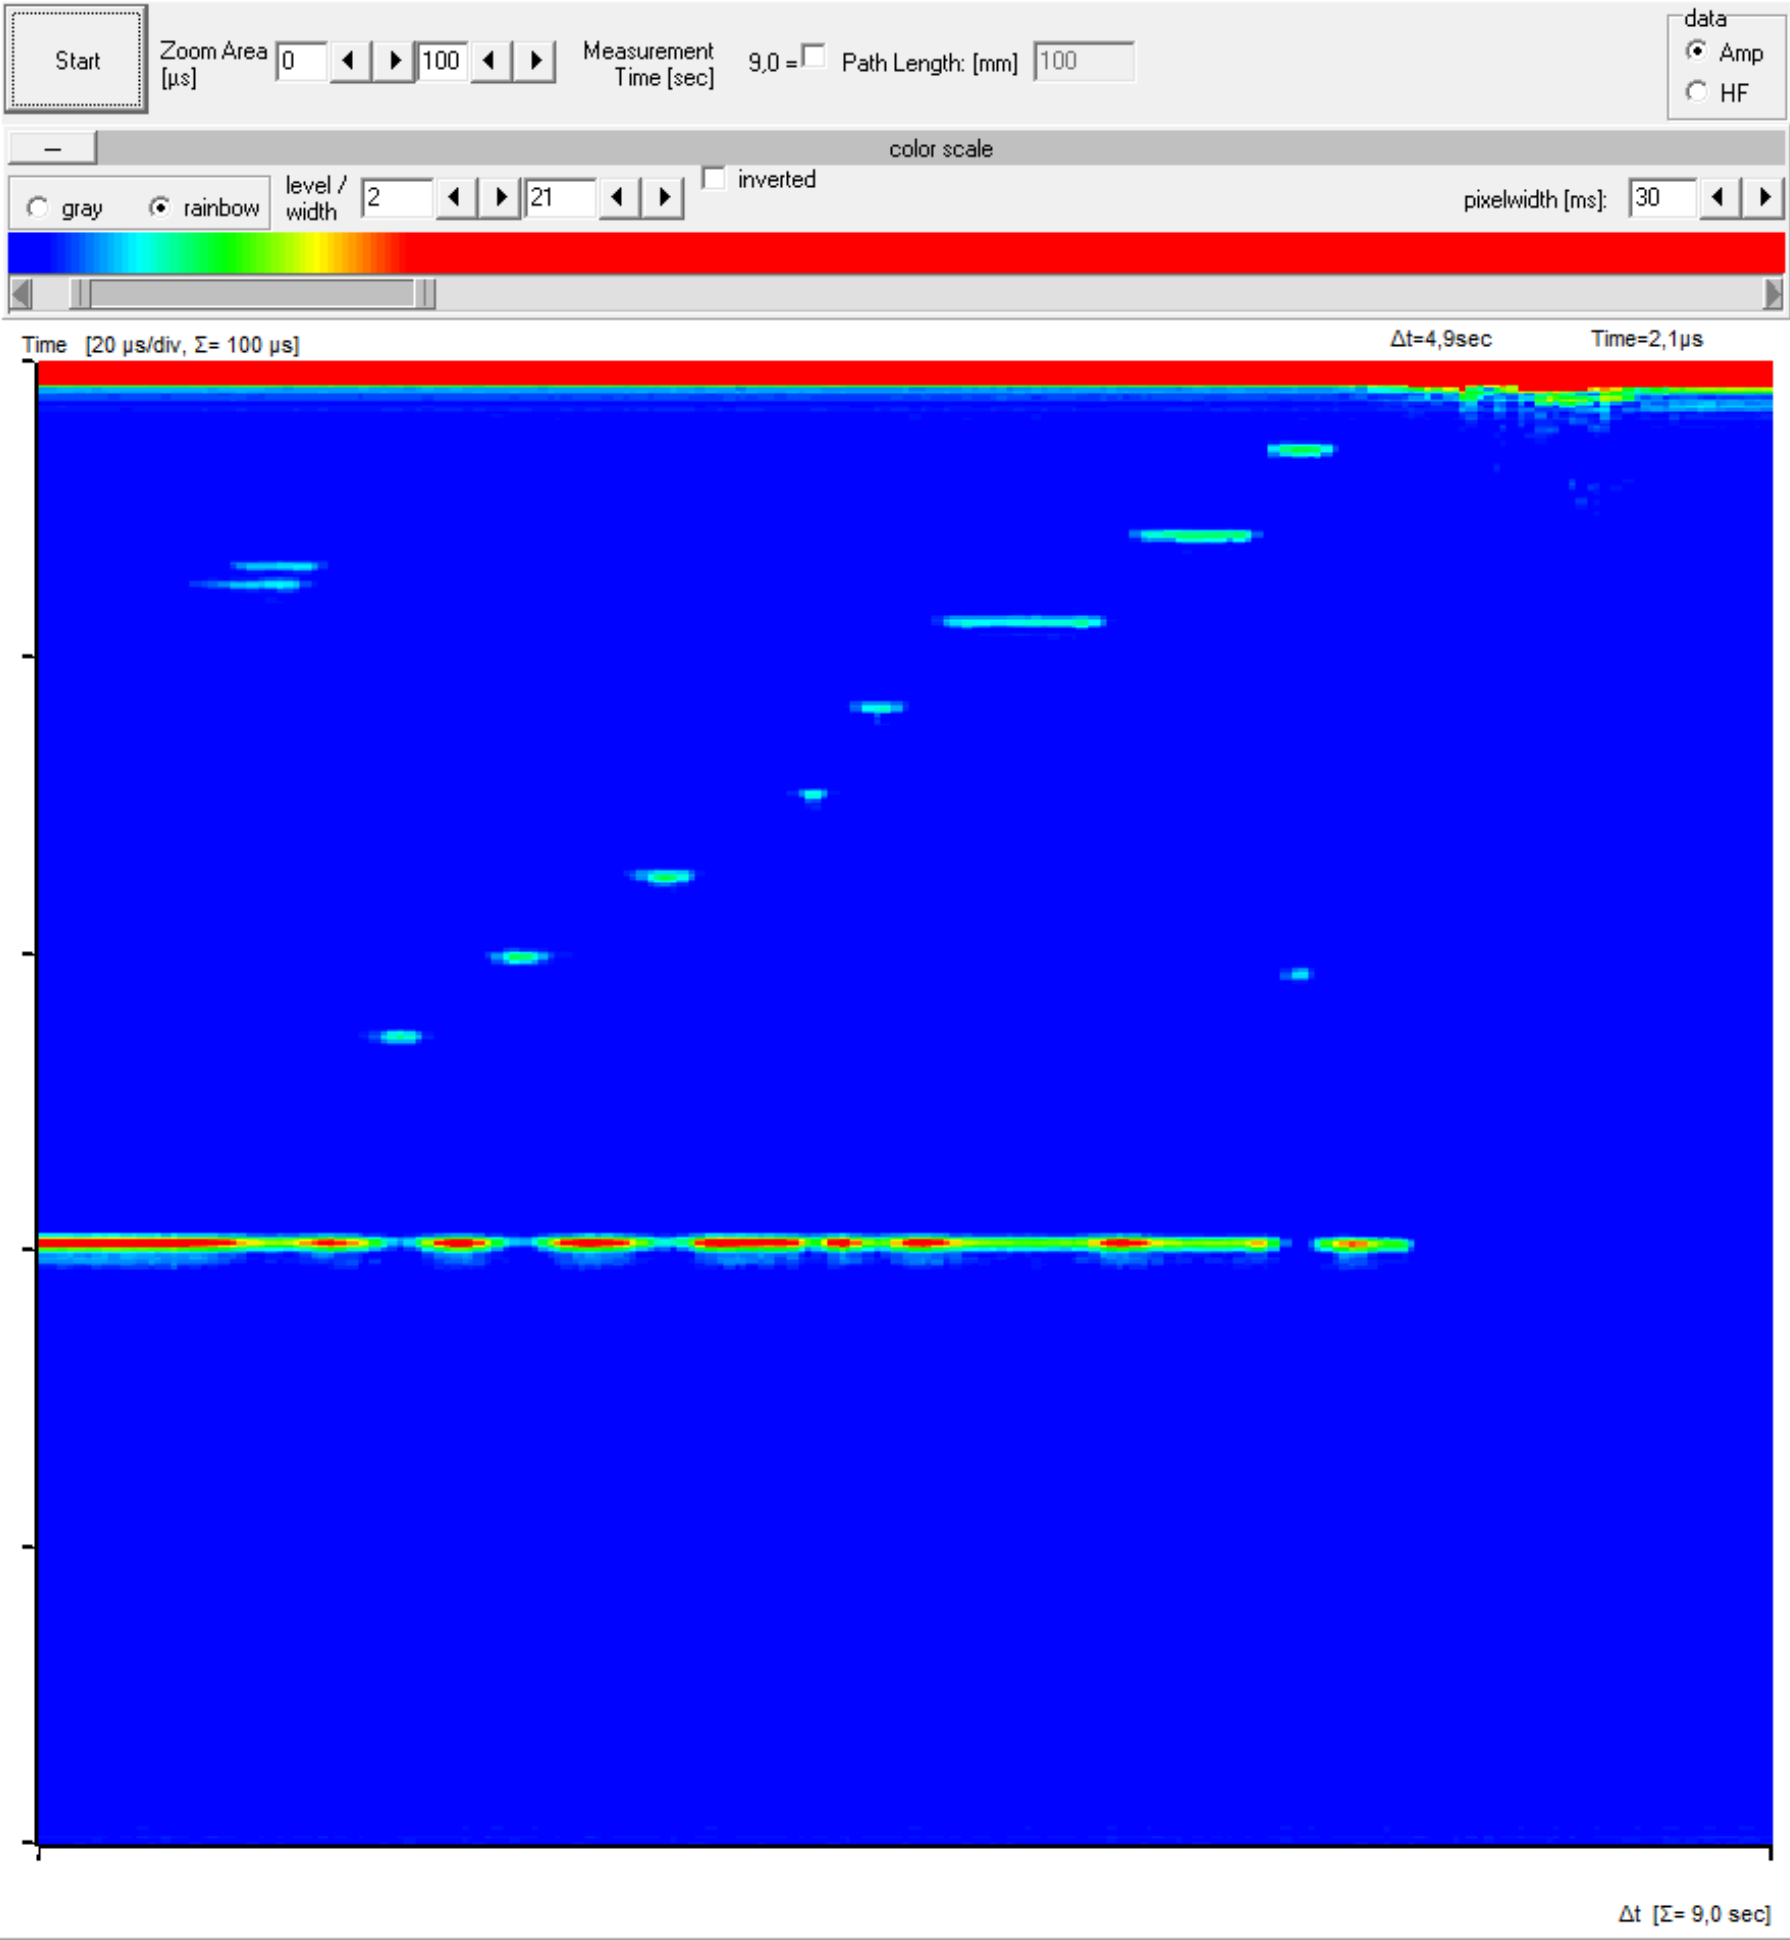
\includegraphics[width=\textwidth]{pictures/bo.png}
  \caption{B-Scan von oben.}
  \label{fig:bo}
  \end{subfigure}
  \hfill
  \begin{subfigure}{0.49\columnwidth}
  \centering
  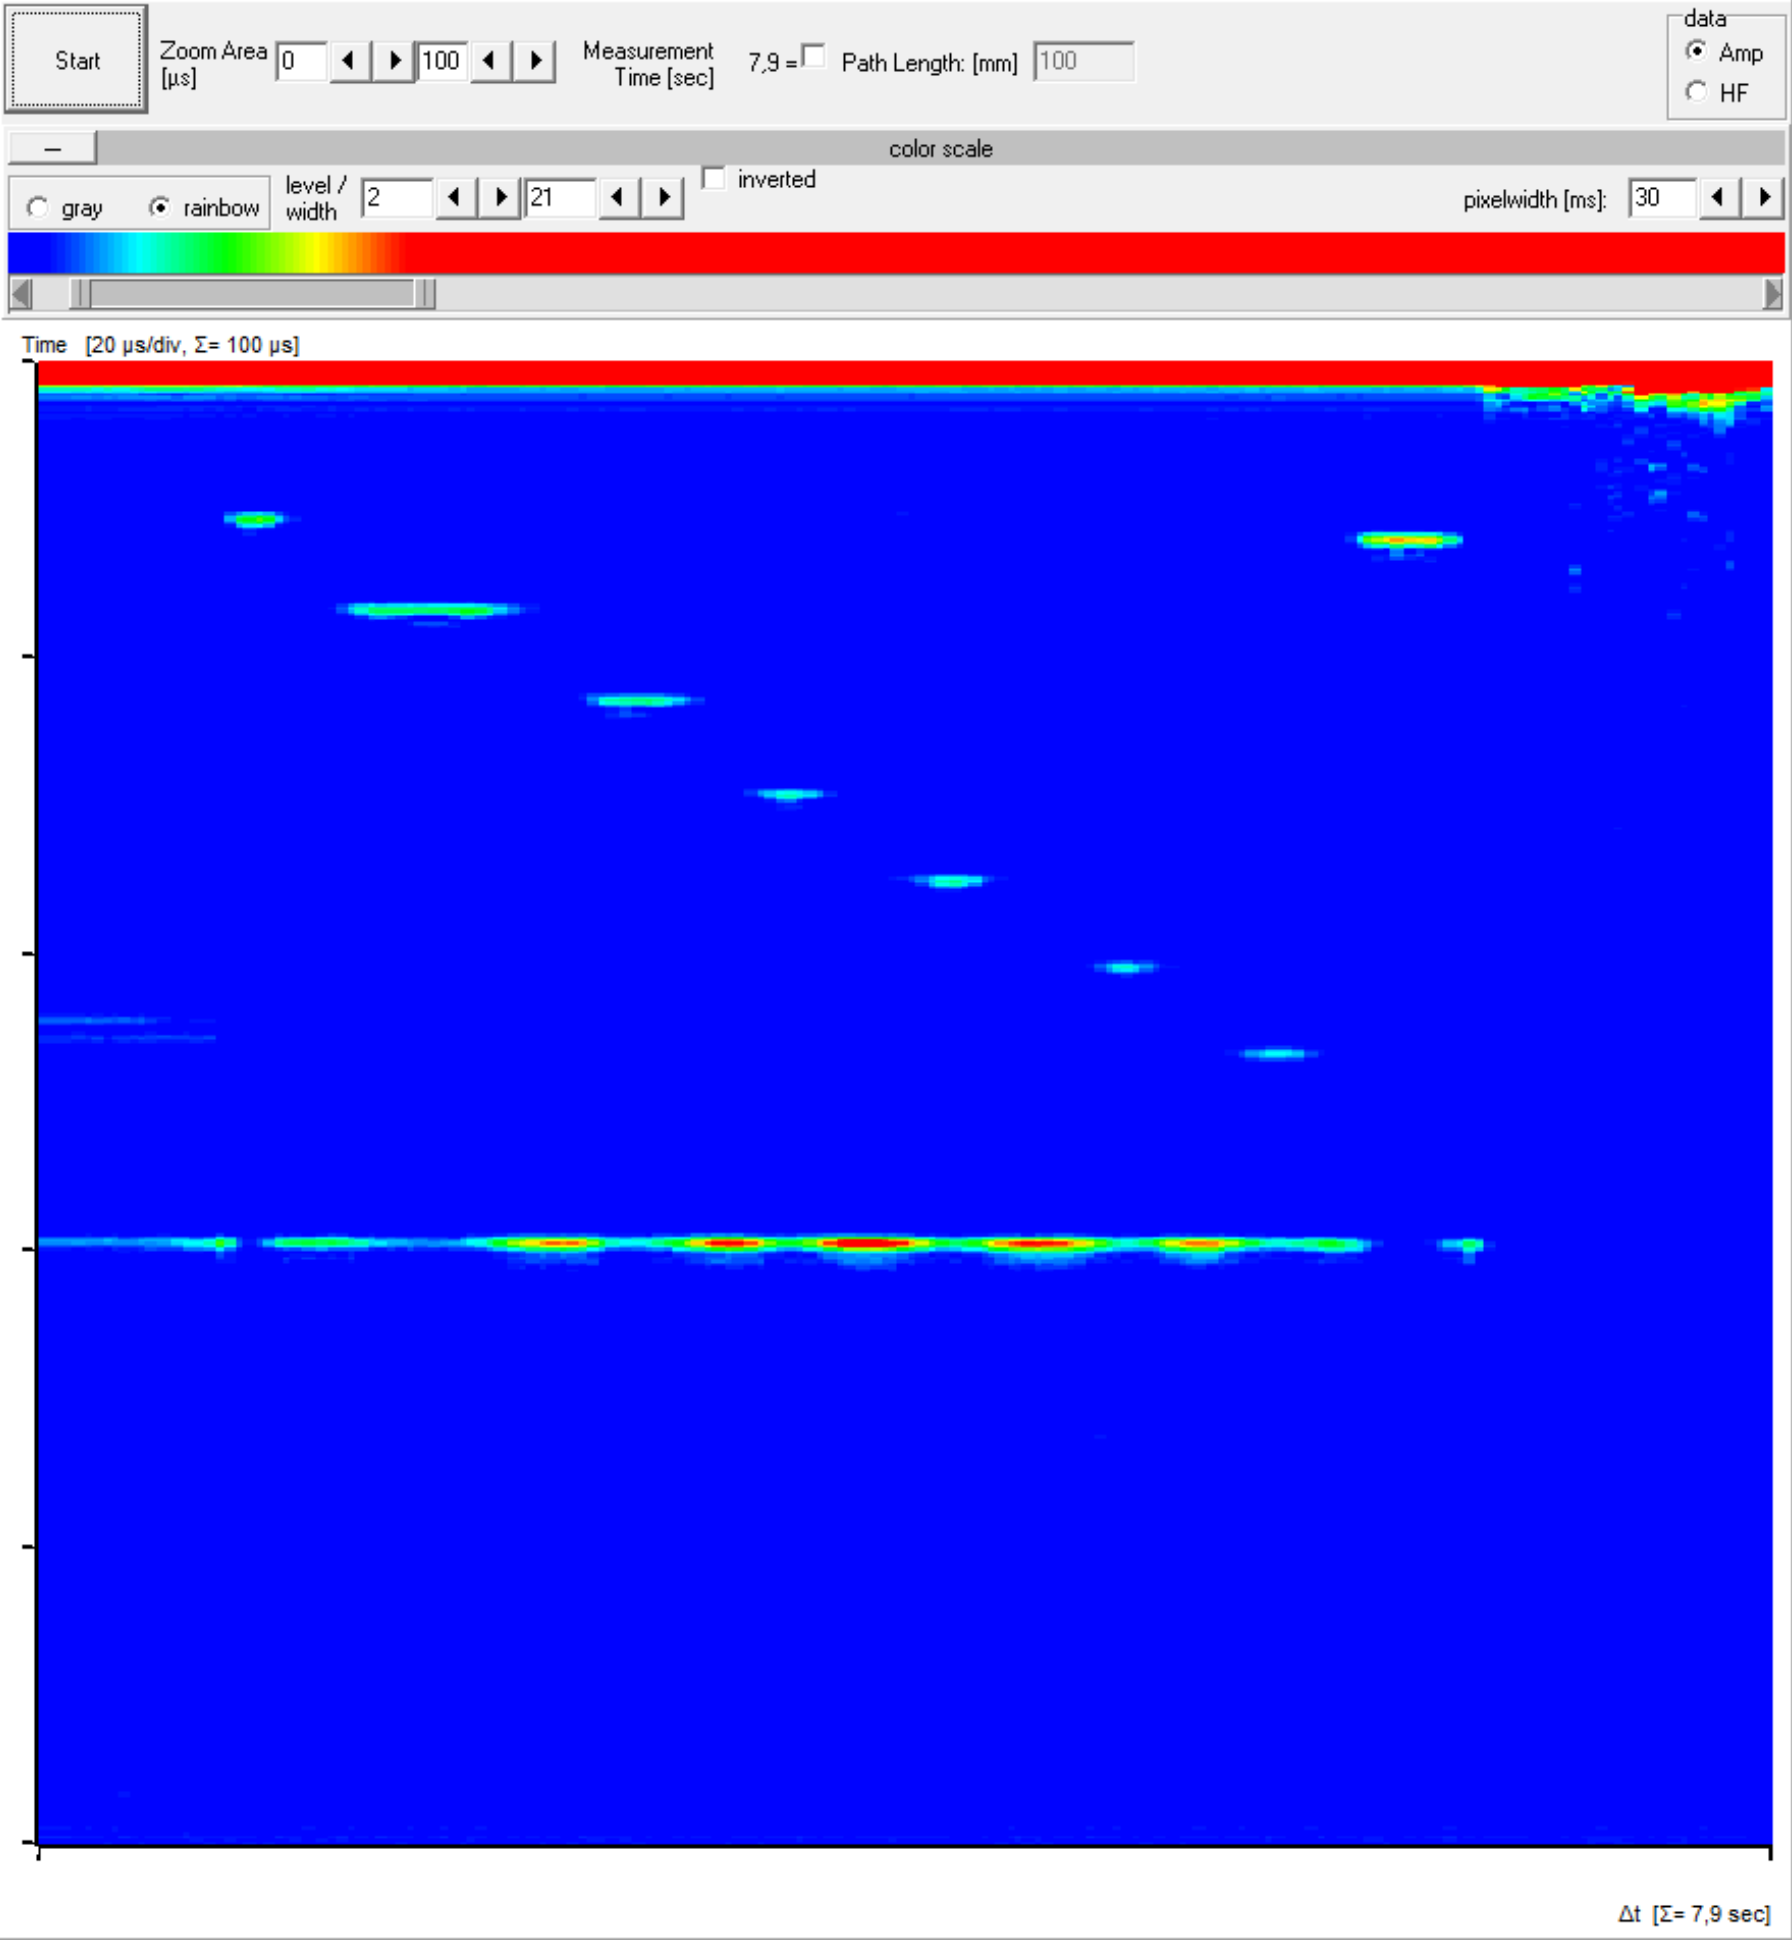
\includegraphics[width=\textwidth]{pictures/bu.png}
  \caption{B-Scan von unten.}
  \label{fig:bu}
  \end{subfigure}

  \caption{B-Scan des Acrylblocks, die Störstellen sind nummeriert von links nach rechts zu erkennen.}
  \label{fig:b-scan}
\end{figure}

Aus beiden Aufnahmen lassen sich ähnlich wie beim A-Scan in \autoref{sec:a-scan} die Laufzeiten ausgehend von der Sonde ablesen.
Daraus werden die Abstände und schließlich die Durchmesser in \autoref{tab:b-scan} berechnen.
\begin{table}[H]
  \centering
  \caption{Die Laufzeiten und die berechneten Werte der Störstellen mittels B-Scan.}
  \label{tab:b-scan}
  \begin{tabular}{c c c c c c}
    \toprule
    \multicolumn{1}{c}{Stelle} &
    \multicolumn{1}{c}{$t_\text{oben} \mathbin{/} \unit{\micro\second}$} &
    \multicolumn{1}{c}{$d_\text{oben} \mathbin{/} \unit{\centi\meter}$} &
    \multicolumn{1}{c}{$t_\text{unten} \mathbin{/} \unit{\micro\second}$} &
    \multicolumn{1}{c}{$d_\text{unten} \mathbin{/} \unit{\centi\meter}$} &
    \multicolumn{1}{c}{$d_\text{Loch} \mathbin{/} \unit{\milli\meter}$ } \\

    \cmidrule(lr){1-1} \cmidrule(lr){2-3} \cmidrule(lr){4-5} \cmidrule(lr){6-6} 
    
      3 &    45,5 &    6,21 &     11,0 &     1,50 &    5,28 \\
      4 &    40,3 &    5,46 &     16,5 &     2,25 &    4,87 \\
      5 &    34,5 &    4,71 &     24,0 &     3,28 &    2,55 \\
      6 &    28,8 &    3,93 &     29,5 &     4,03 &    2,82 \\
      7 &    23,3 &    3,18 &     35,2 &     4,80 &    2,55 \\
      8 &    17,3 &    2,36 &     41,0 &     5,60 &    2,82 \\
      9 &    11,4 &    1,56 &     47,0 &     6,42 &    2,68 \\
     10 &     5,5 &    0,75 &        - &        - &       - \\
     11 &    41,5 &    5,66 &     12,0 &     1,64 &    9,37 \\
    \bottomrule
  \end{tabular}
\end{table}


\subsection{Bestimmung der Lage und Größe der Tumore im Brustmodell}

Nach Ertasten des Brustmodells lasst sich der eine Tumor in oberer und der andere in rechter Lage bestimmen.
Für beide Tumore werden A-Scans mit jeweils der $\qty{1}{MHz}$- und der $\qty{2}{MHz}$-Sonde durchgeführt, 
diese sind in \autoref{fig:boob_oben} und \autoref{fig:boob_rechts} dargestellt.
\begin{figure}
  \centering
  
  \begin{subfigure}{0.49\columnwidth}
  \centering
  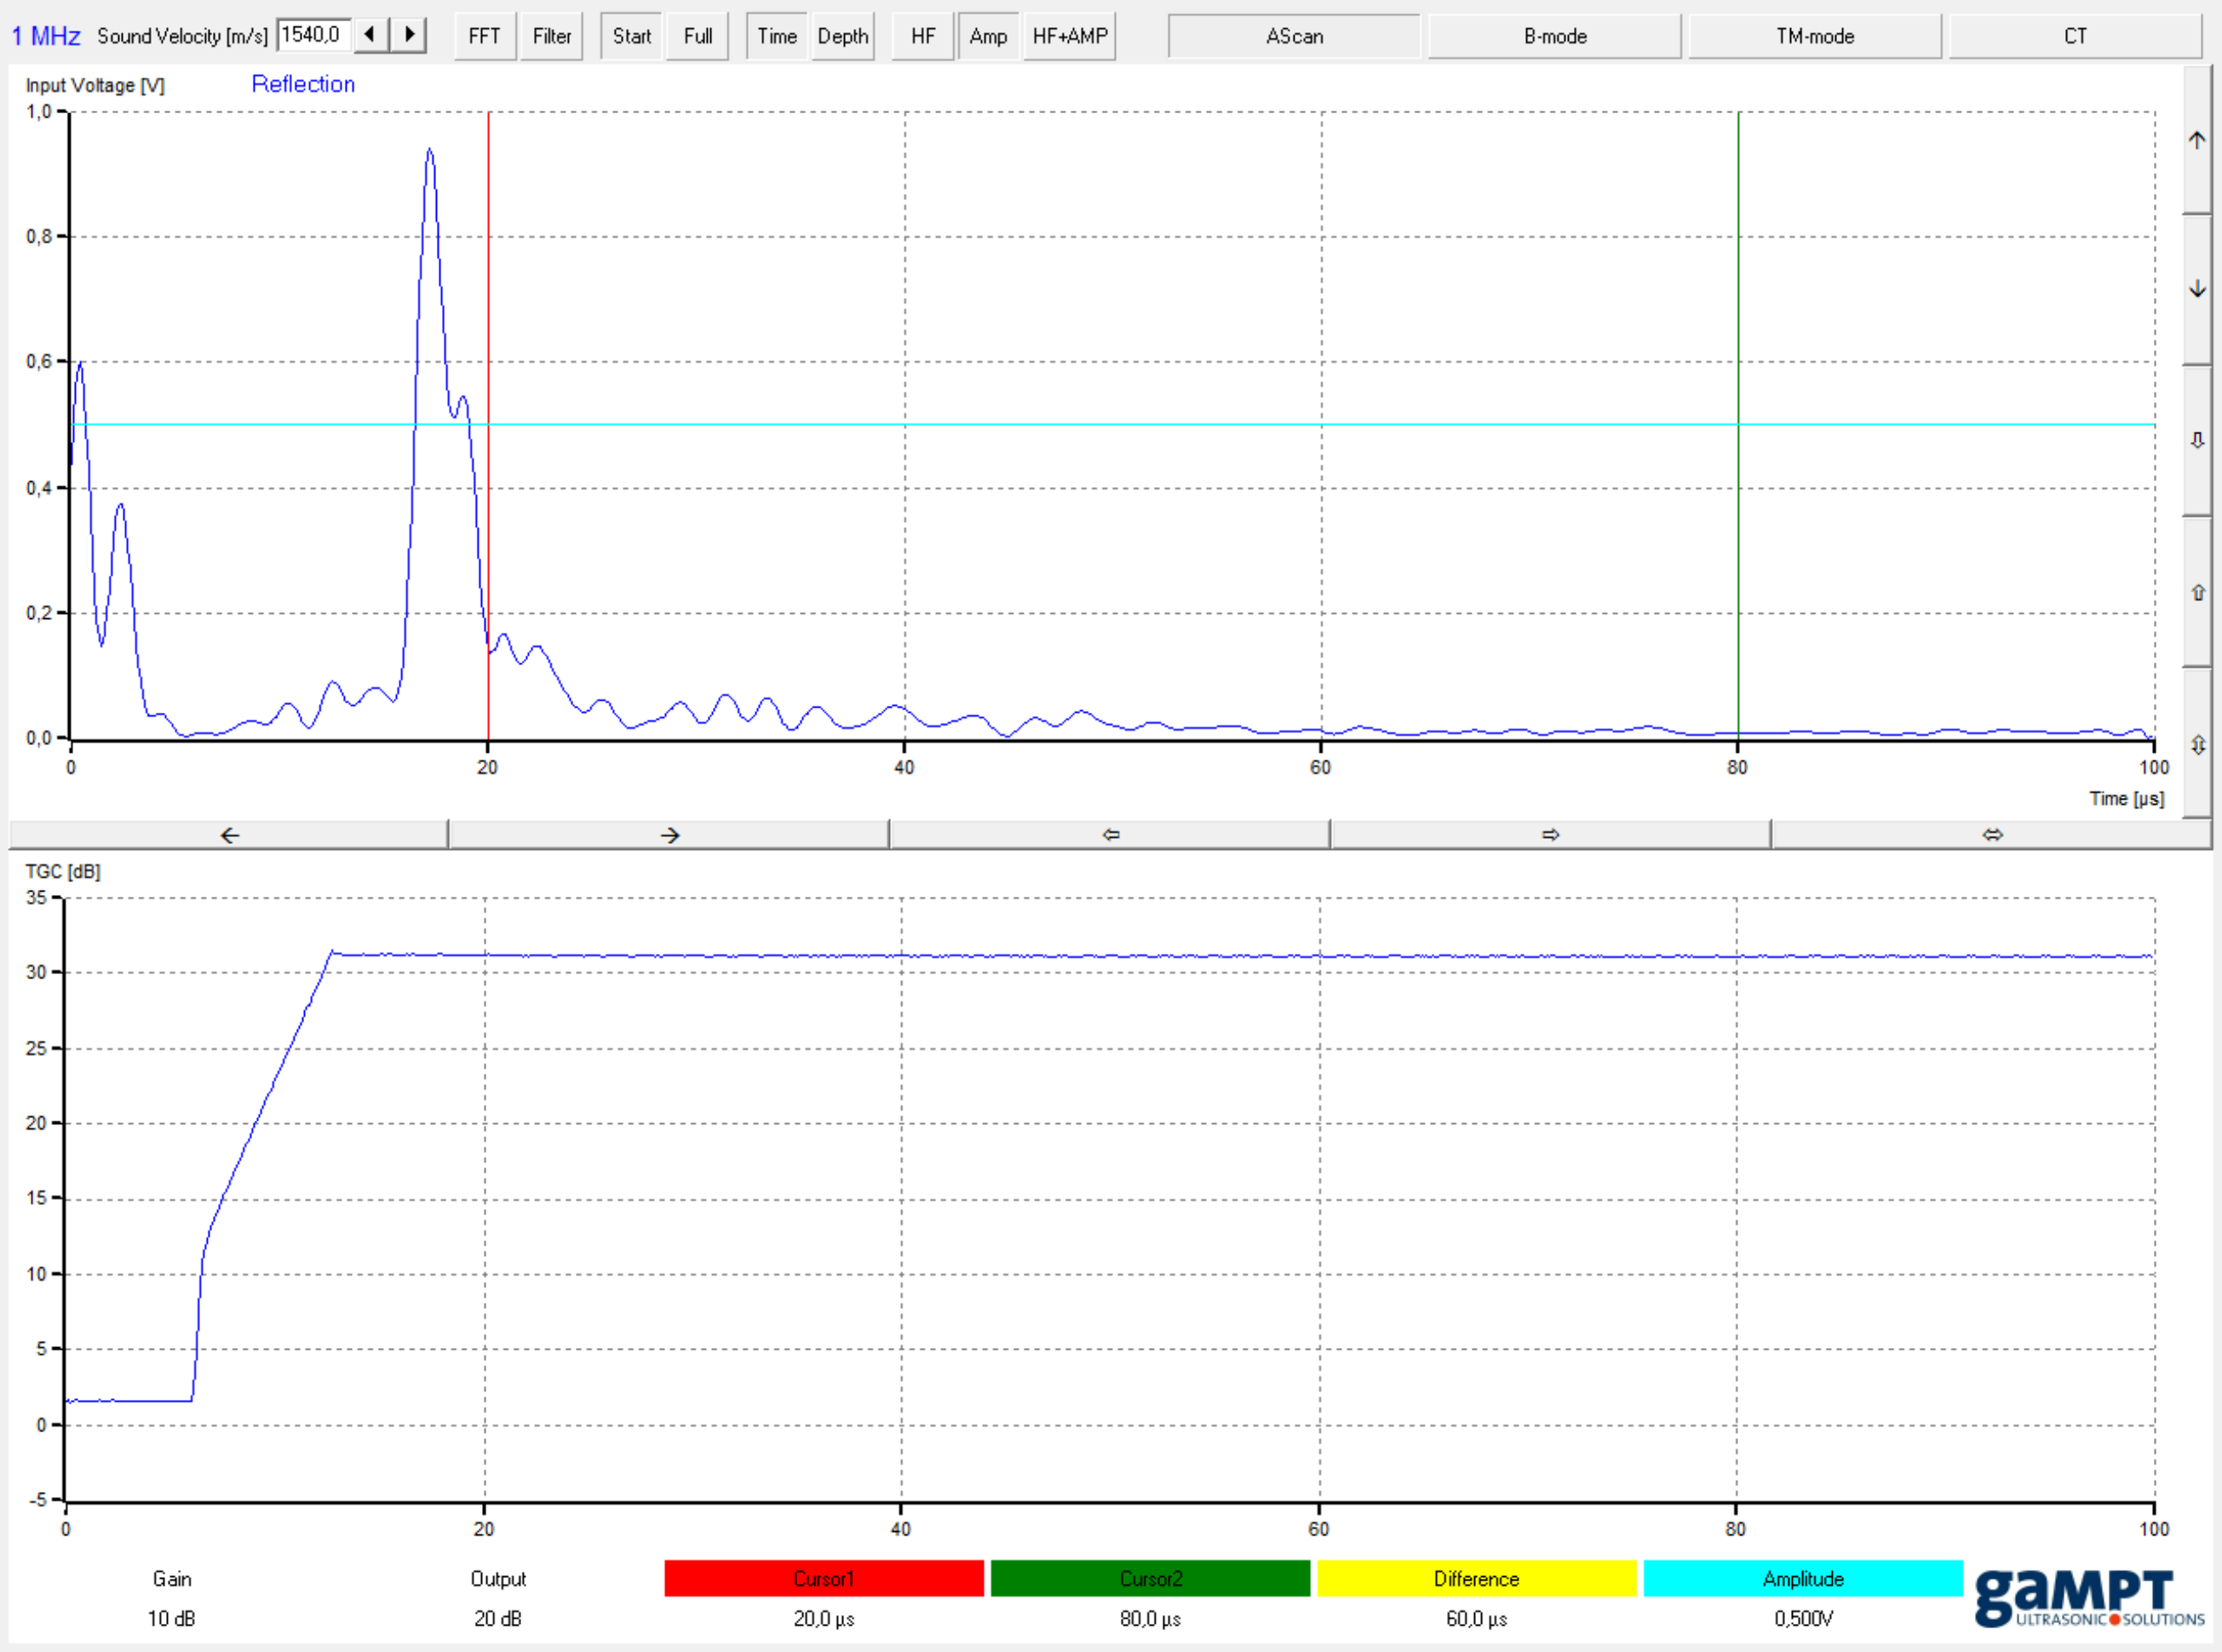
\includegraphics[width=\textwidth]{pictures/boob_oben_1MHz.png}
  \caption{A-Scan mit der $\qty{1}{MHz}$-Sonde.}
  \label{fig:boob_oben_1}
  \end{subfigure}
  \hfill
  \begin{subfigure}{0.49\columnwidth}
  \centering
  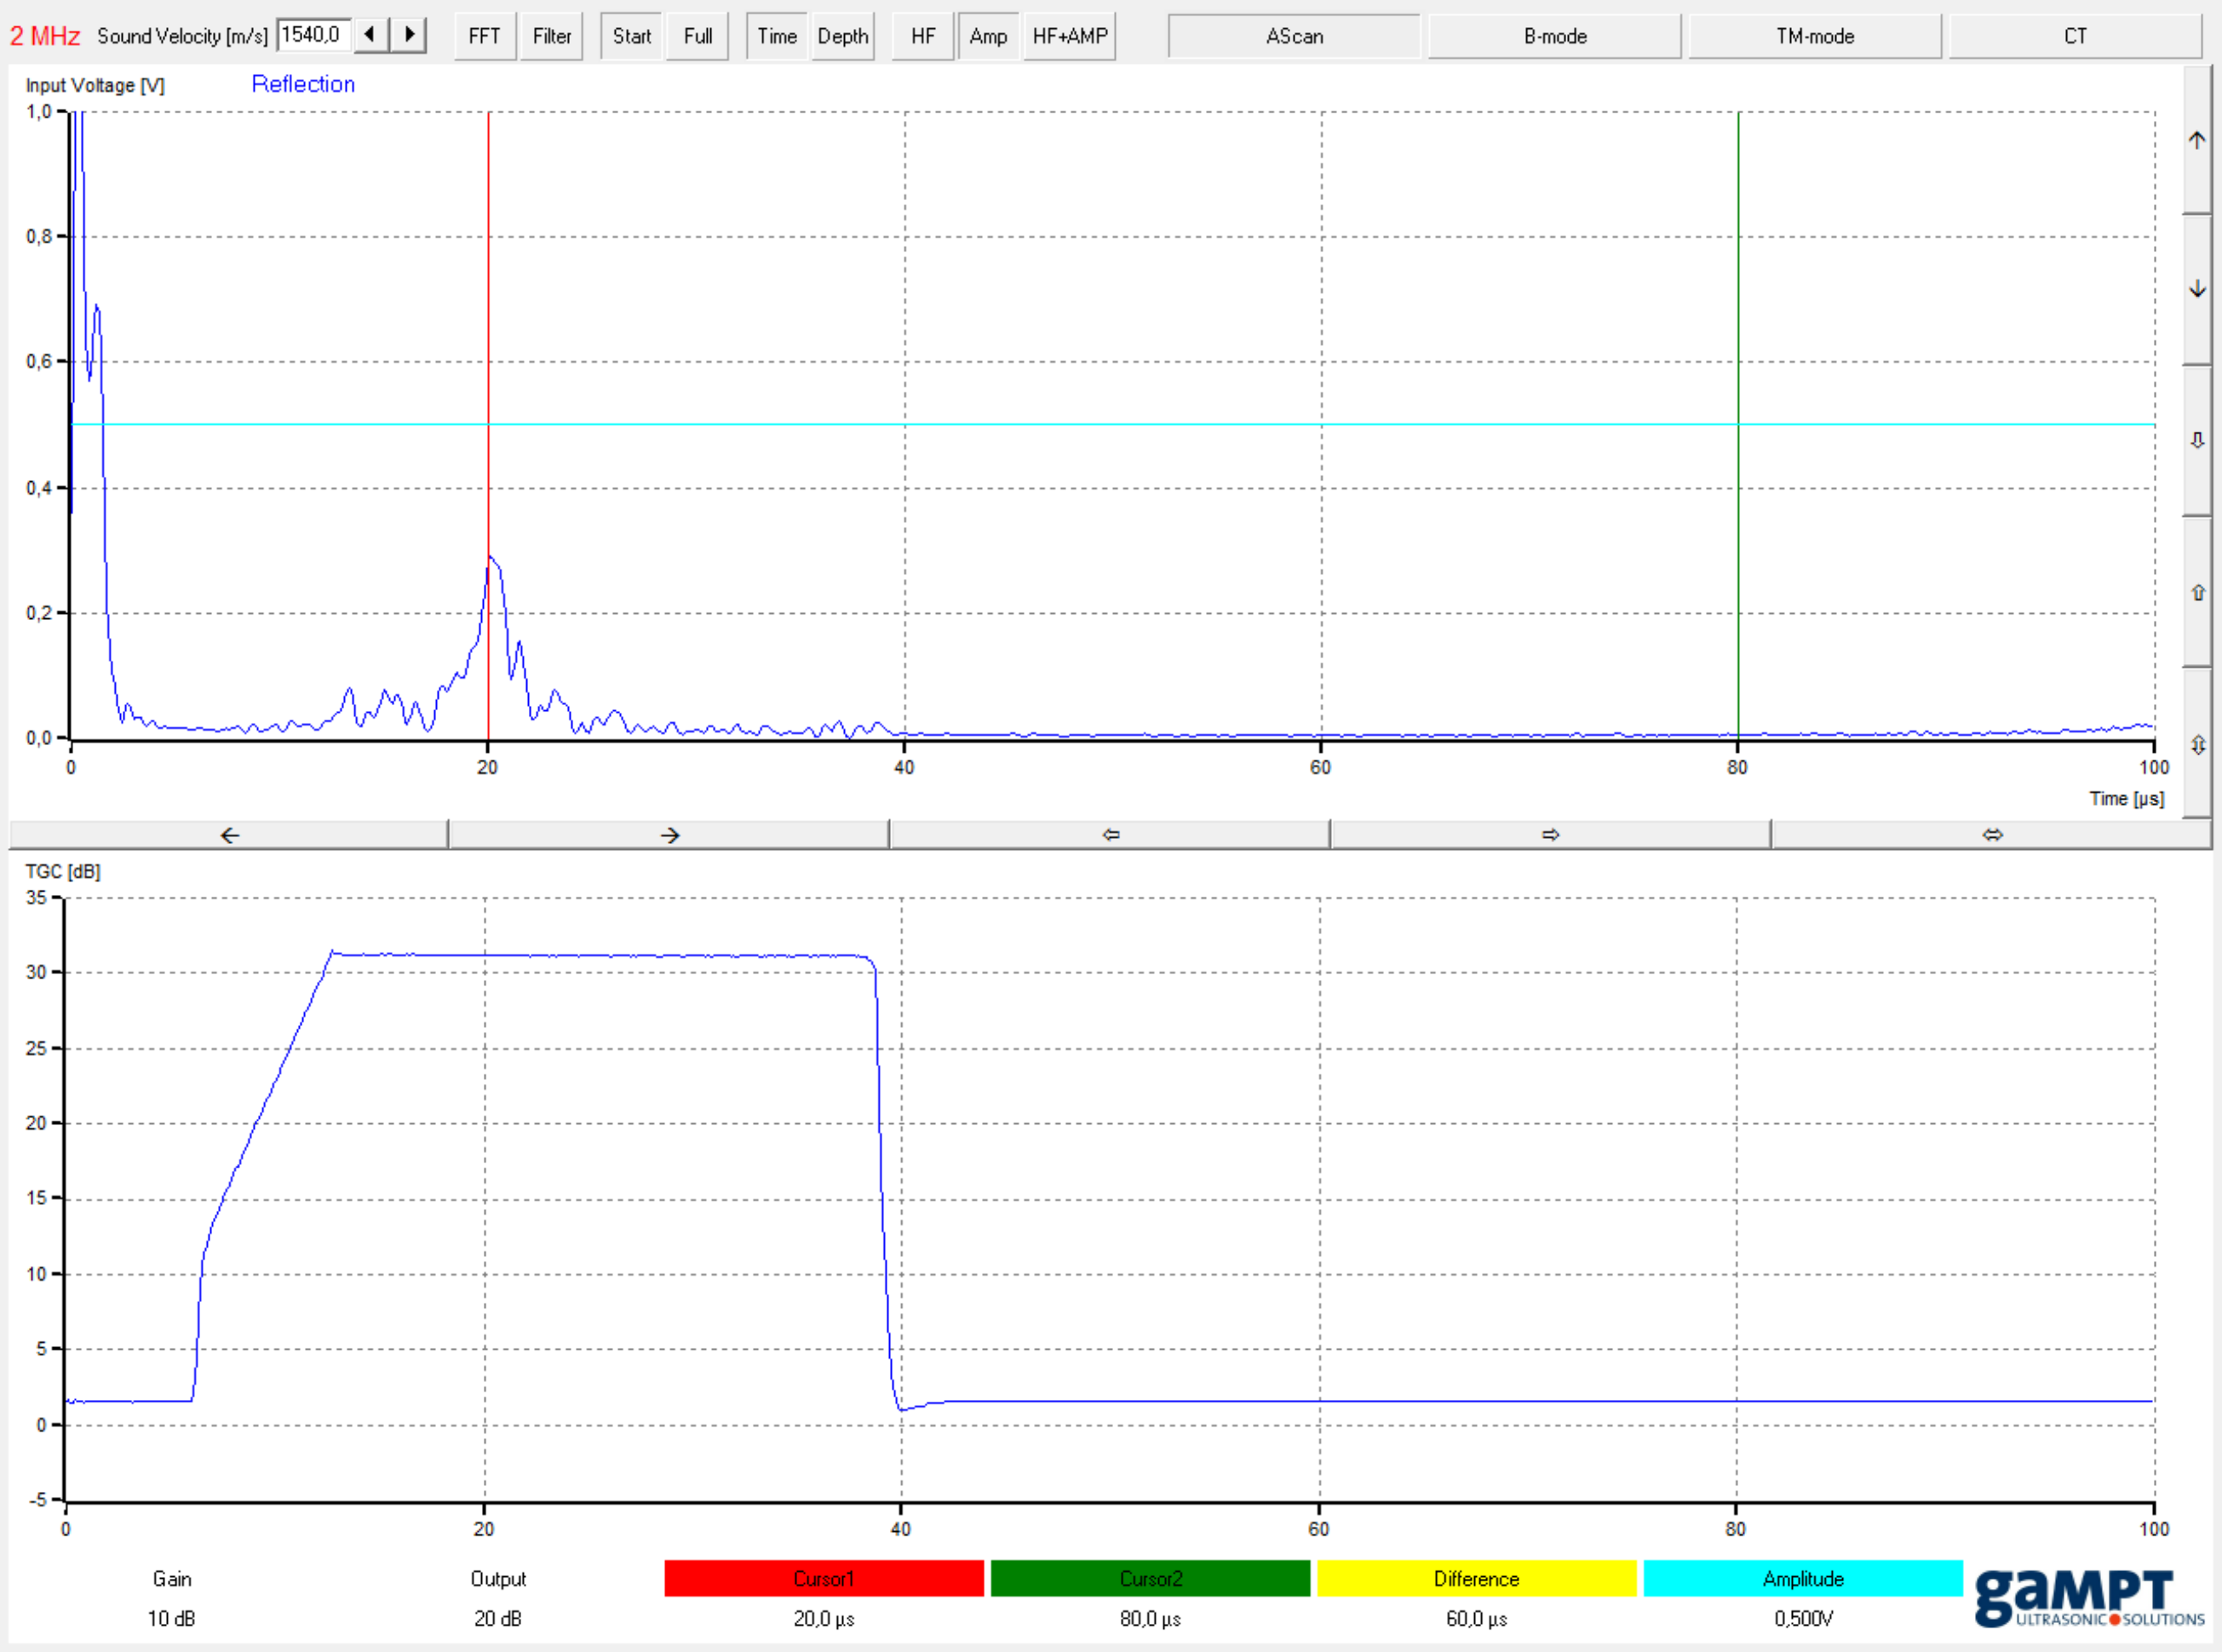
\includegraphics[width=\textwidth]{pictures/boob_oben_2MHz.png}
  \caption{A-Scan mit der $\qty{2}{MHz}$-Sonde.}
  \label{fig:boob_oben_2}
  \end{subfigure}

  \caption{Der A-Scan des oberen Bereichs für die $\qty{1}{MHz}$- und $\qty{2}{MHz}$-Sonde.}
  \label{fig:boob_oben}
\end{figure}

\begin{figure}
  \centering
  
  \begin{subfigure}{0.49\columnwidth}
  \centering
  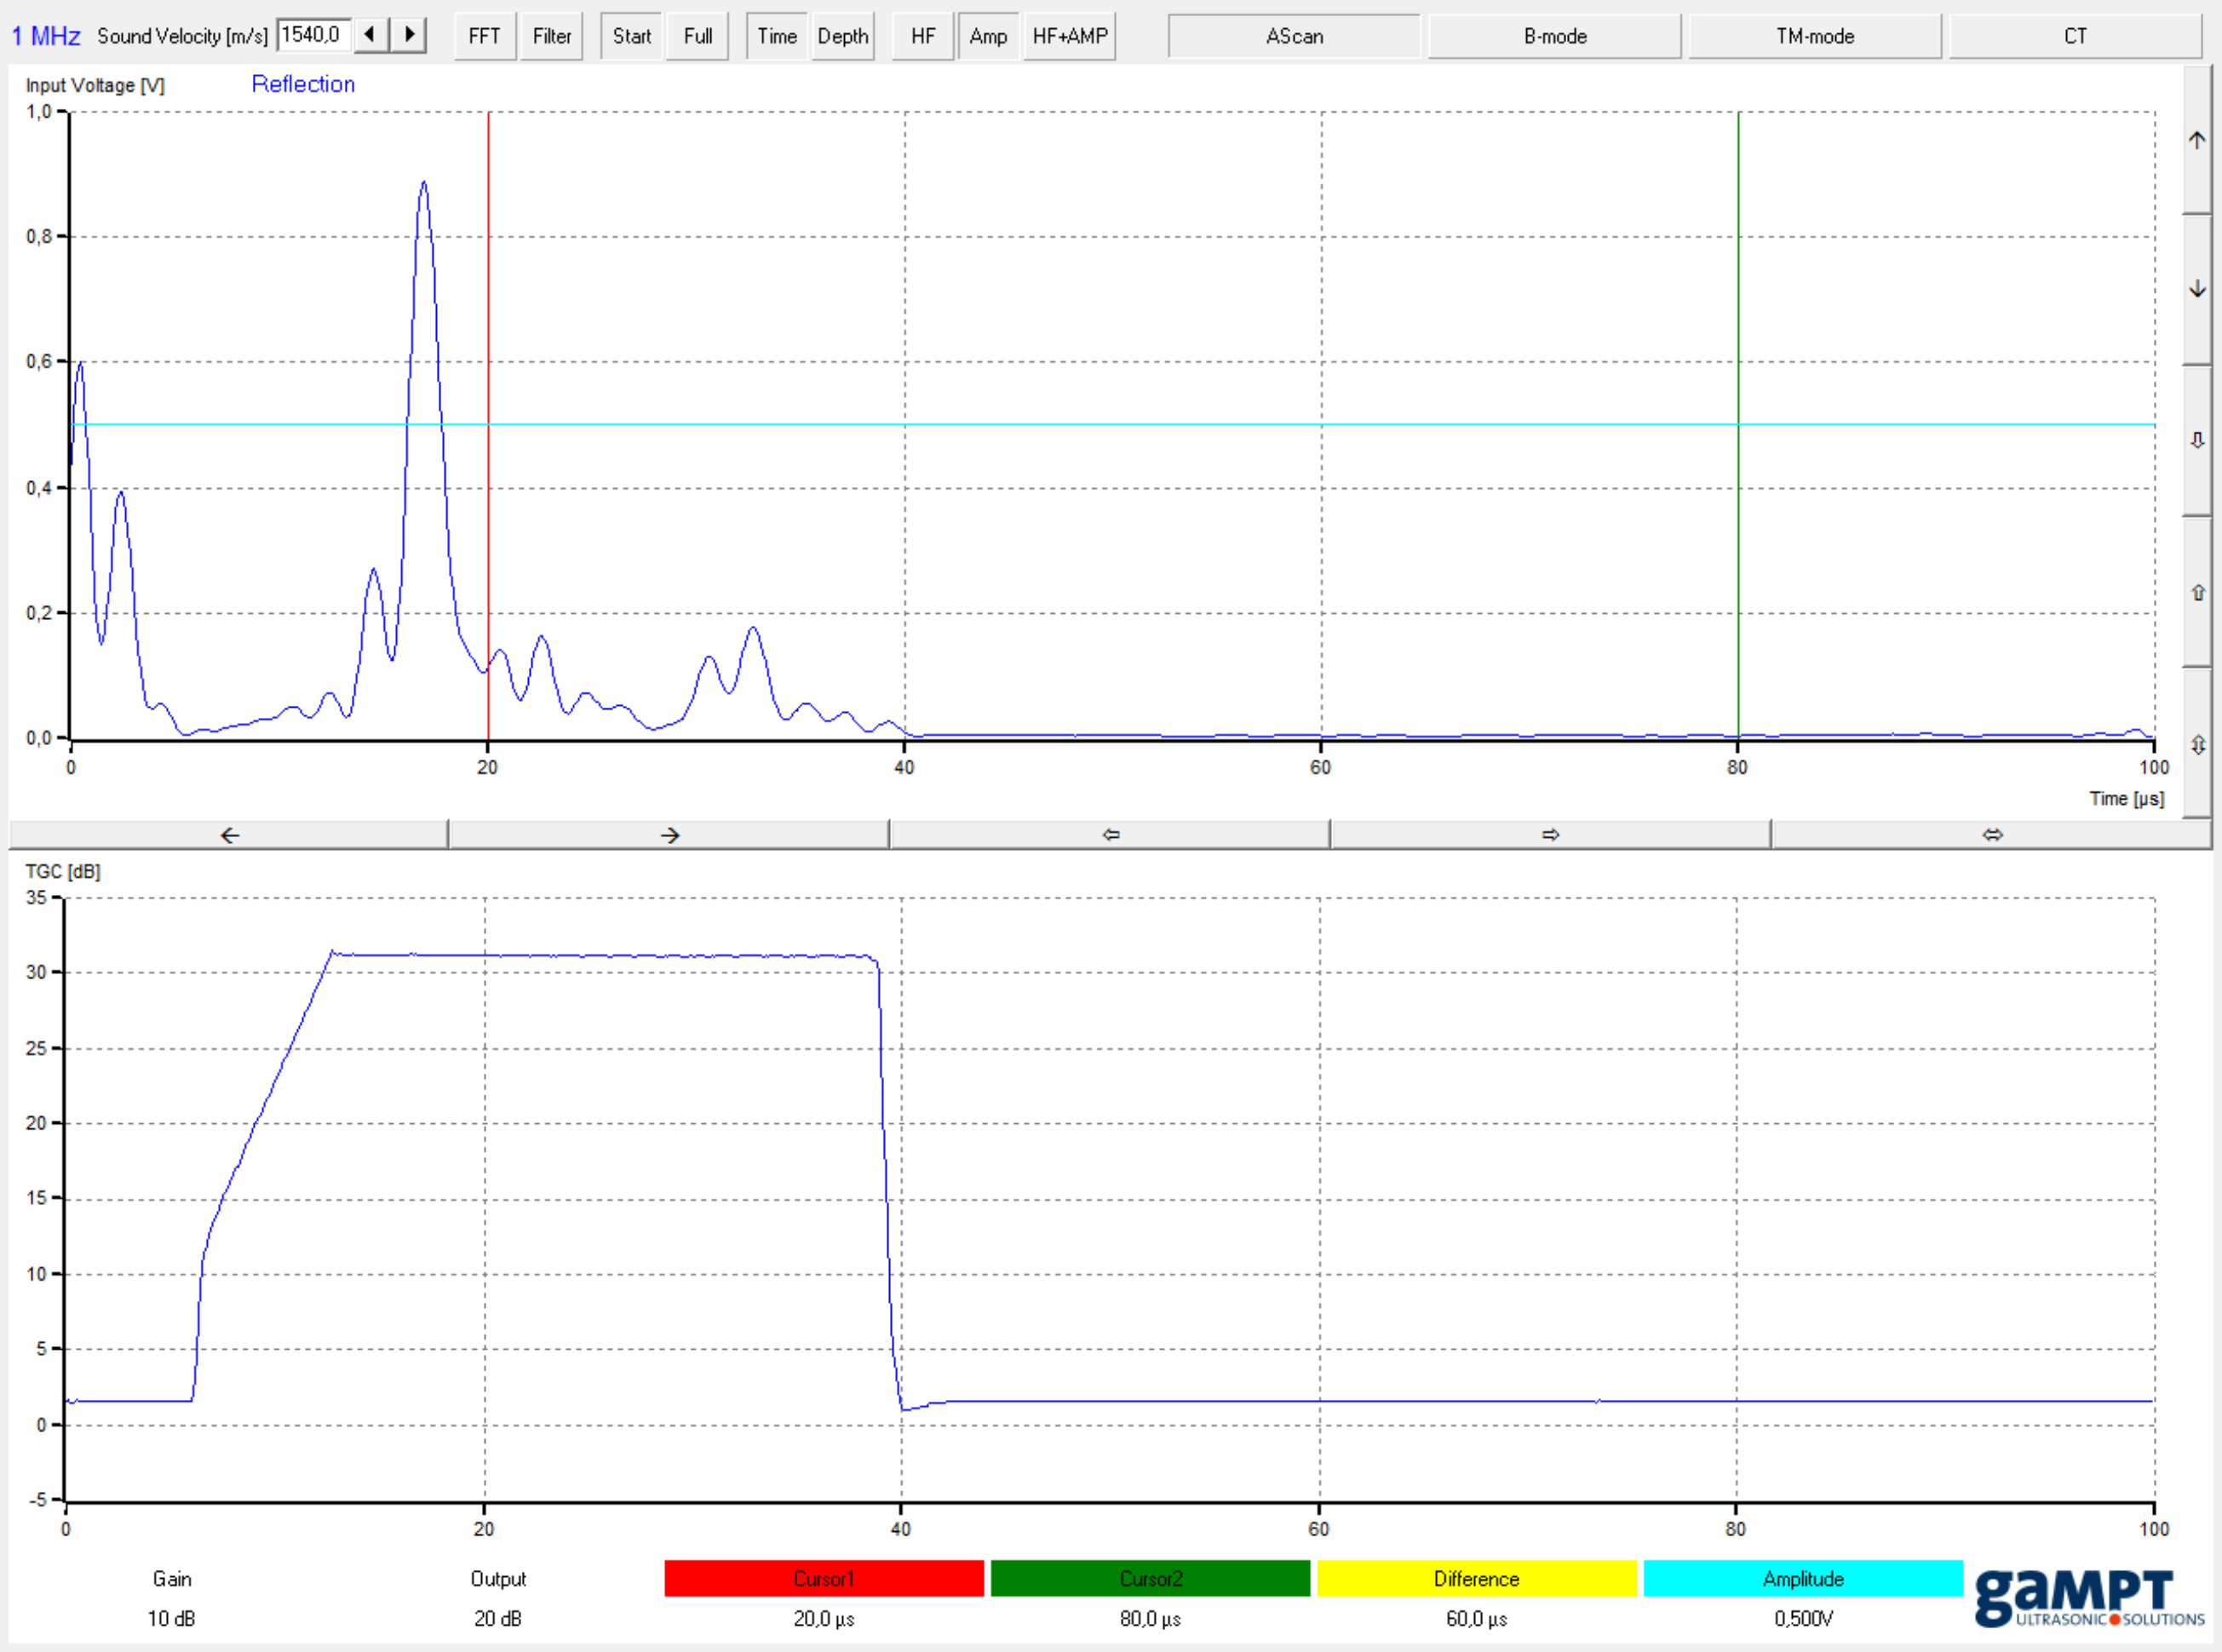
\includegraphics[width=\textwidth]{pictures/boob_rechts_1MHz.png}
  \caption{A-Scan mit der $\qty{1}{MHz}$-Sonde.}
  \label{fig:boob_rechts_1}
  \end{subfigure}
  \hfill
  \begin{subfigure}{0.49\columnwidth}
  \centering
  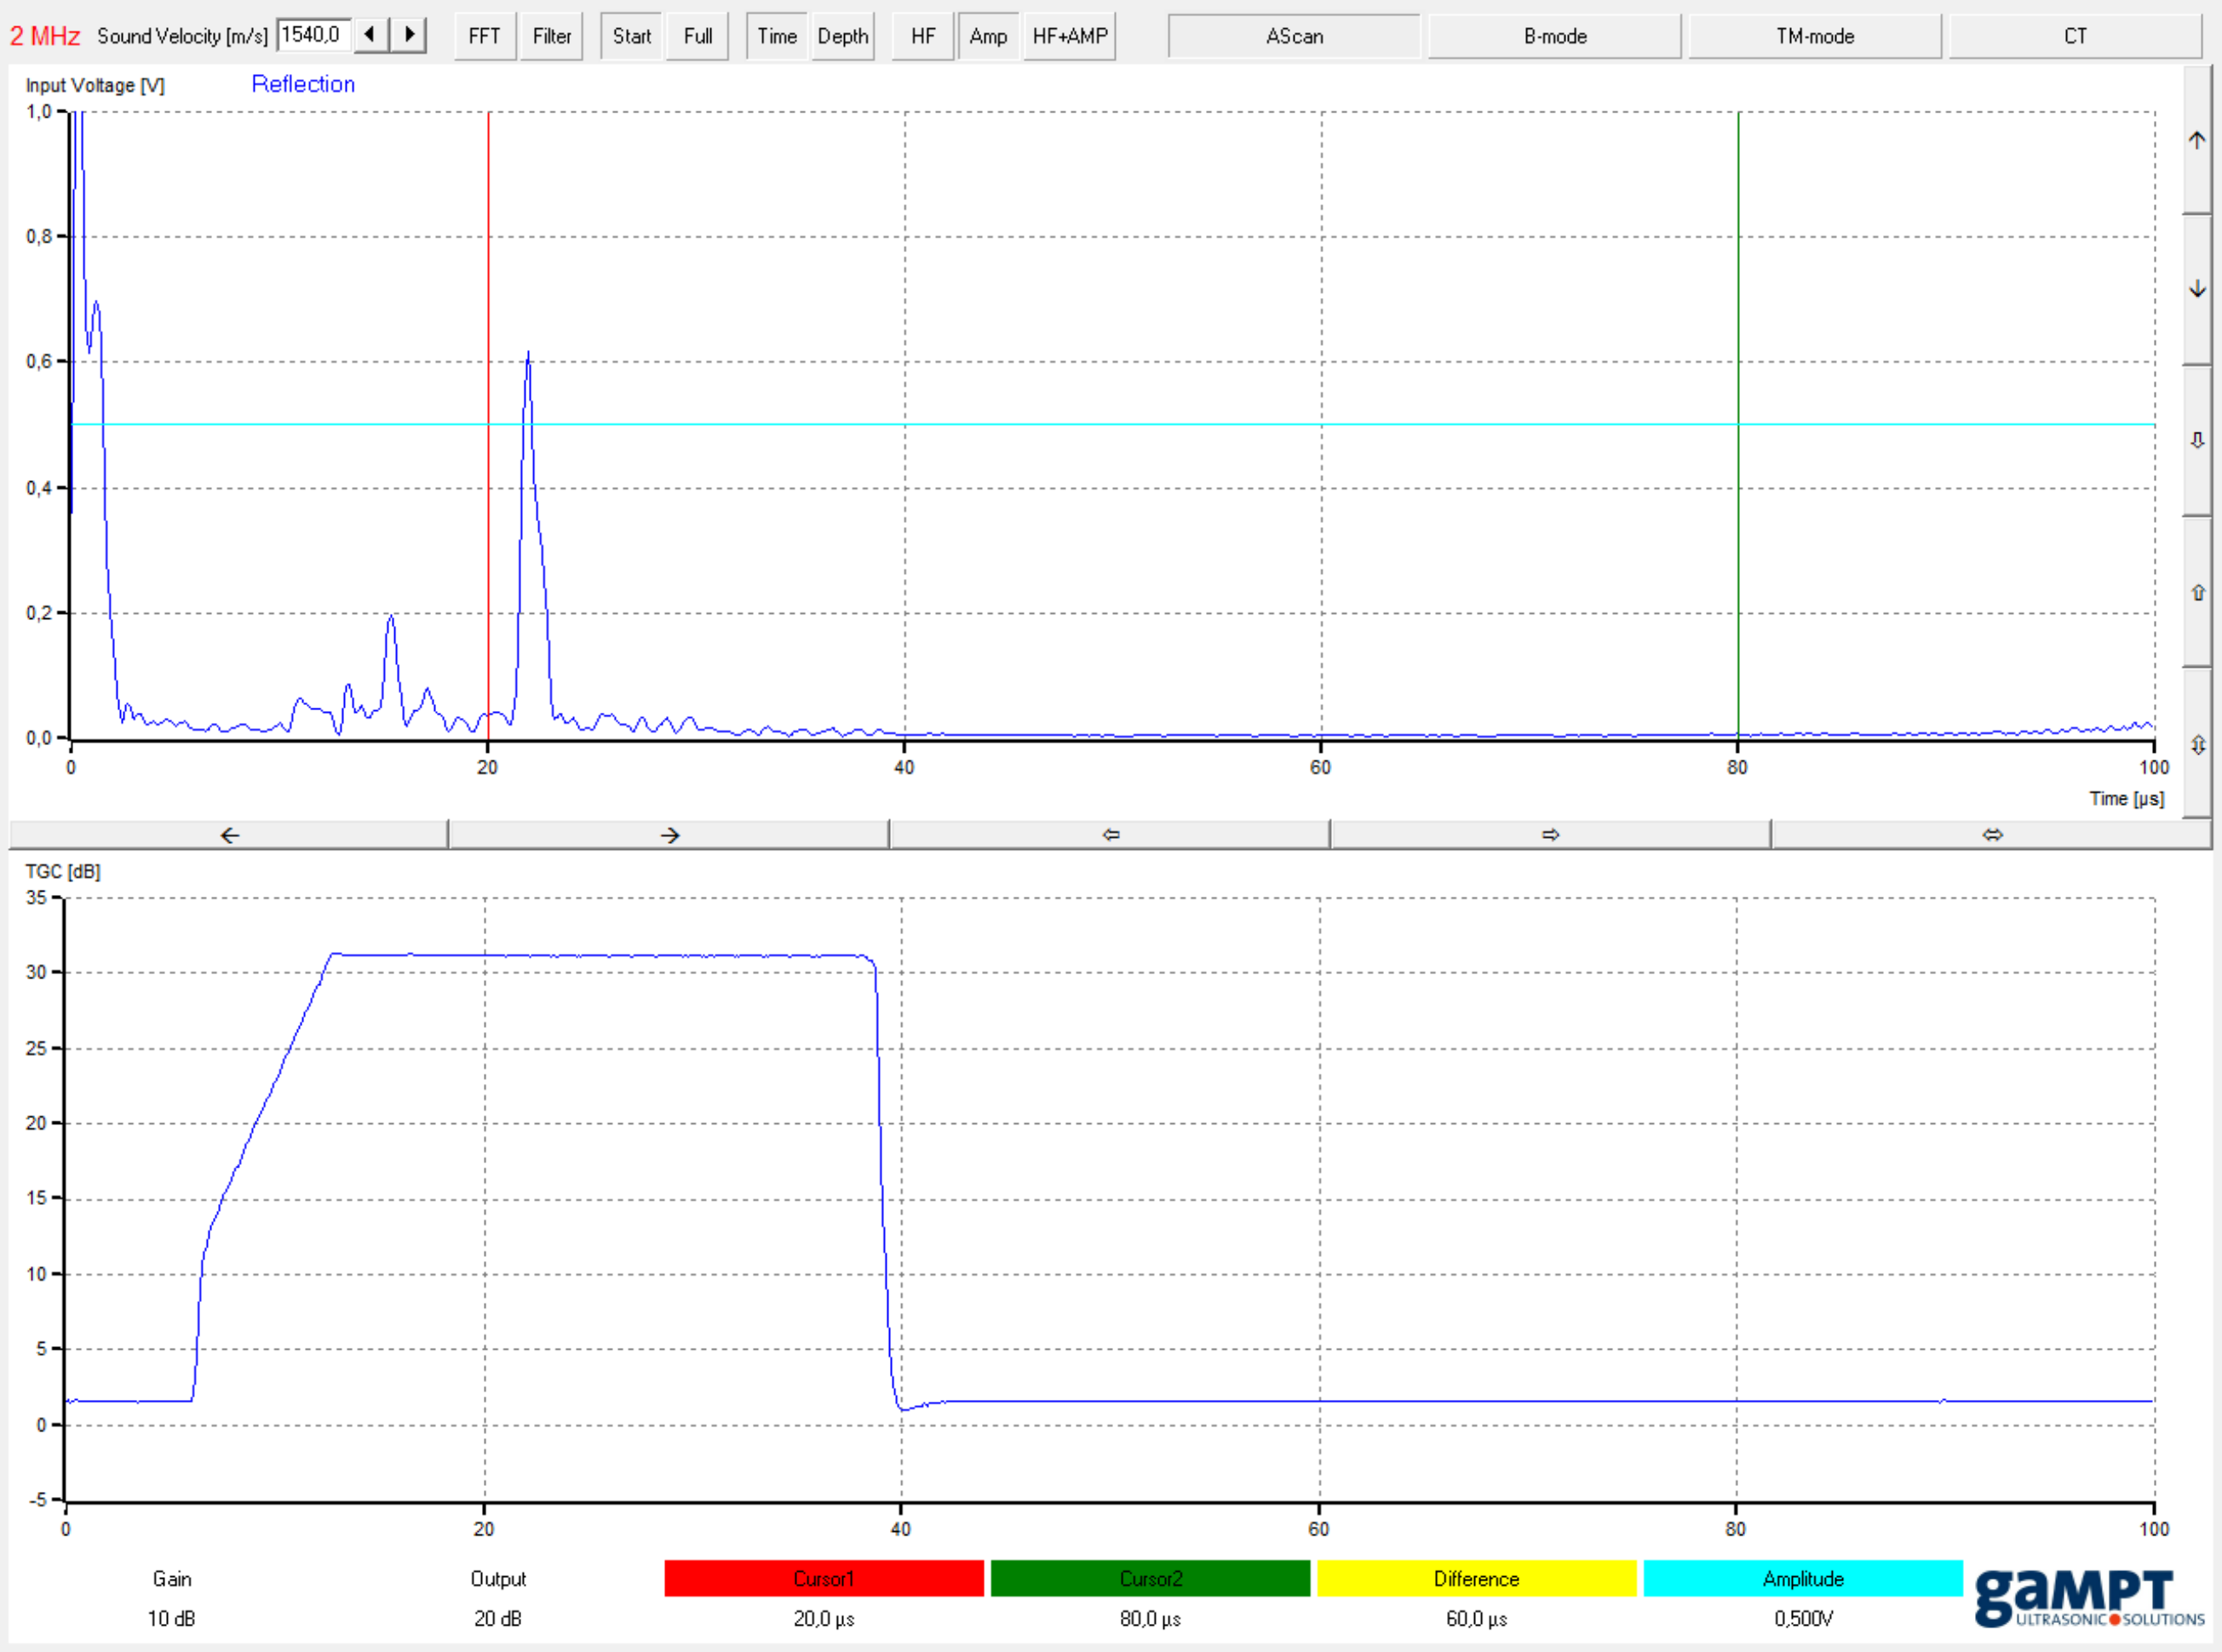
\includegraphics[width=\textwidth]{pictures/boob_rechts_2MHz.png}
  \caption{A-Scan mit der $\qty{2}{MHz}$-Sonde.}
  \label{fig:boob_rechts_2}
  \end{subfigure}

  \caption{Der A-Scan des rechten Bereichs für die $\qty{1}{MHz}$- und $\qty{2}{MHz}$-Sonde.}
  \label{fig:boob_rechts}
\end{figure}